\section{Kurzbeschreibung}
Mit dieser Anleitung könnt ihr euren eigenen Malroboter bauen!\\
Dabei wird aus Pappe ein Arm gebaut, welcher mithilfe von zwei Motoren einen Stift über ein Blatt Papier bewegt. Die Motoren werden von einem \textsc{Raspberry-Pi} angesteuert und ihre Geschwindigkeit kann durch einfache Programmierbefehle verändert werden.\\

Die ursprüngliche Idee des Projektes stammt \href{https://tuduu.org/projekt/automatischer-malroboter}{hierher}\footnote[1]{https://tuduu.org/projekt/automatischer-malroboter}. Da ein \textsc{Calliope} teuer und damit vielleicht nicht unbedingt zur Hand ist, haben wir dieses Projekt beispielhaft mit einem \textsc{Raspberry Pi} umgesetzt. Das erfordert zwar einige Zwischenschritte mehr, funktioniert aber mindestens genauso gut.\\

\subsection{Ziel}
Mit diesem Projekt soll den TeilnehmerInnen ein leichter Einstieg in die Programmierung einfacher Elektronik ermöglicht werden.\\



\section{Vorbereitung}
Je nach Durchführung sowie verfügbarer Zeit sollten einige Schritte des Aufbaus vor Projektbeginn erledigt werden, z.B. die Verdrahtung der Motoren (siehe Anhang).\\

\begin{figure}[h]
\centering
\parbox{5cm}{
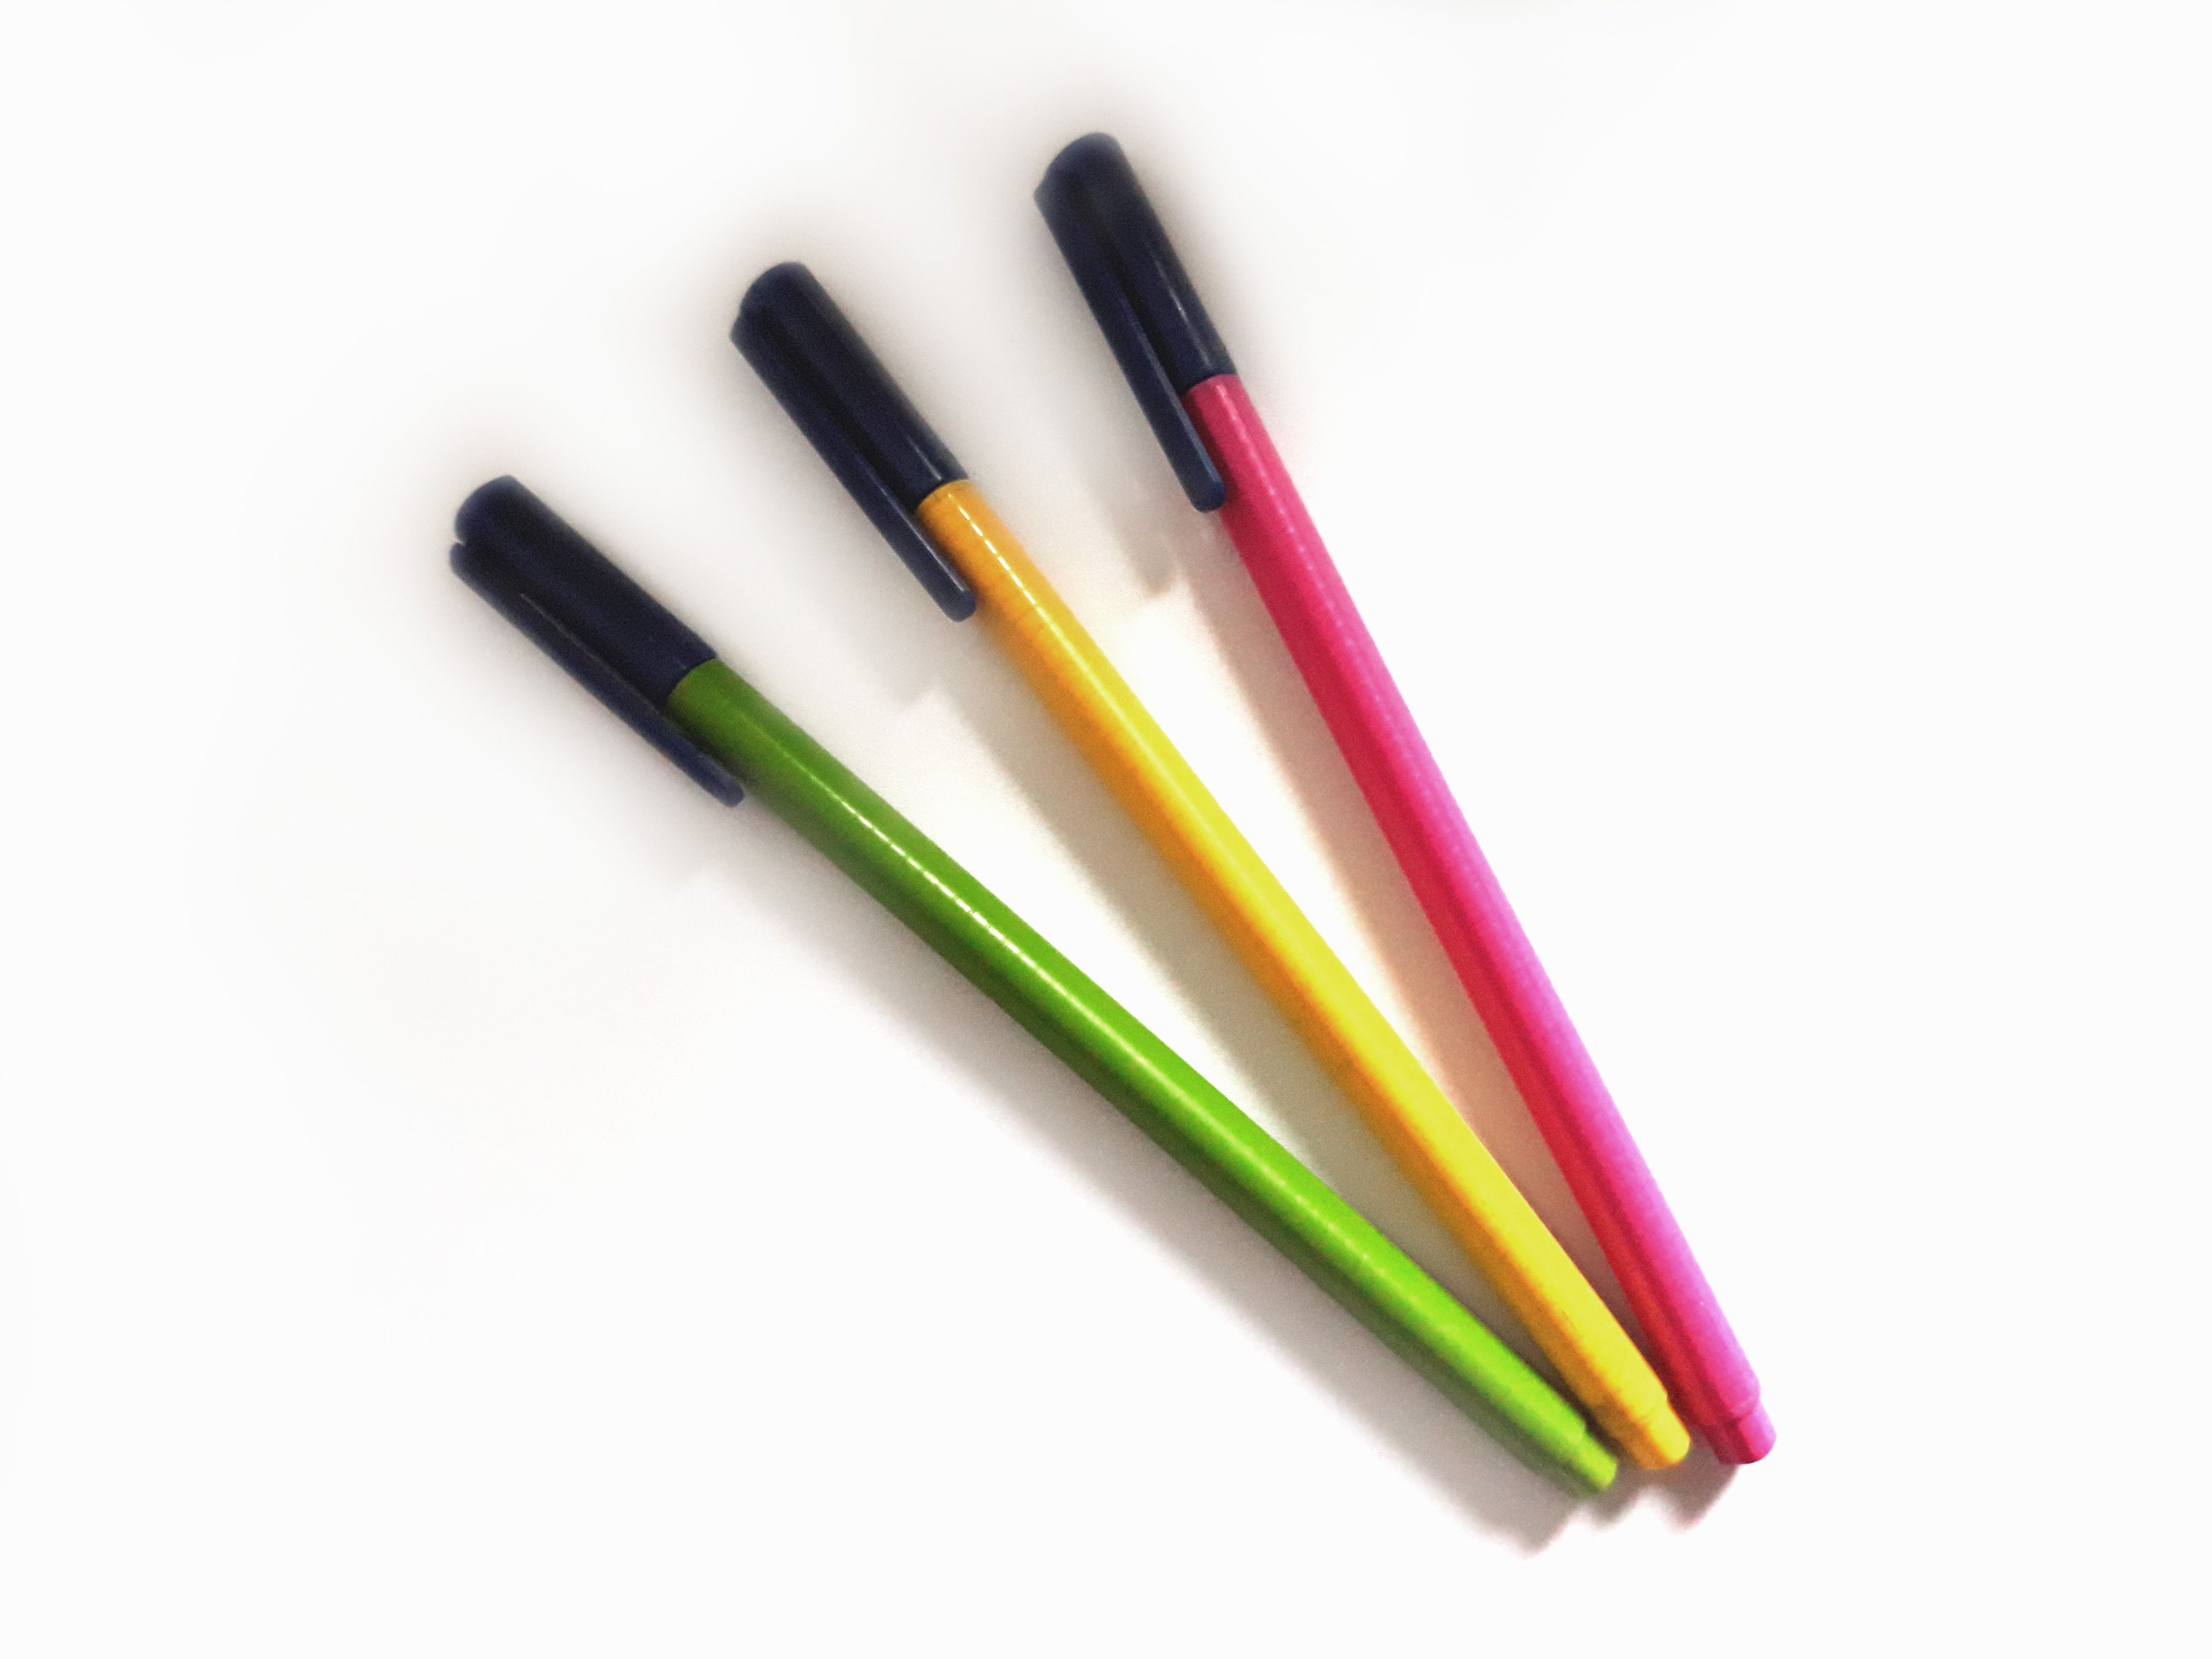
\includegraphics[width=5cm]{stift.jpg}
\caption*{Stifte}s
}
\hfill
\begin{minipage}{5cm}
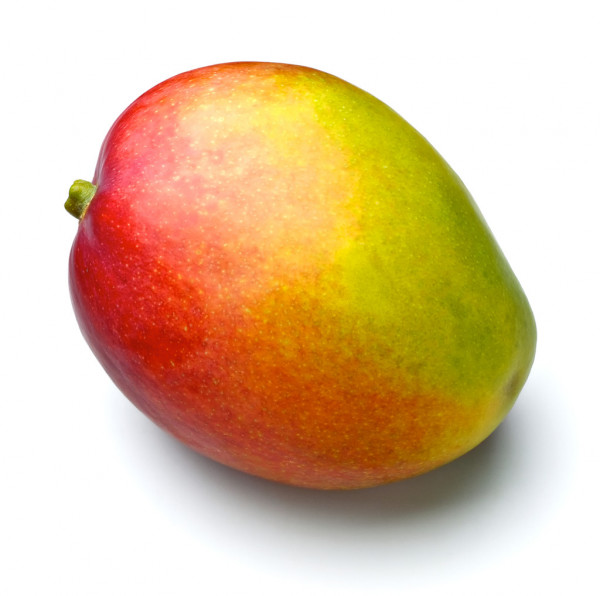
\includegraphics[width=5cm]{mango.jpg}
\caption*{Mango 2}
\end{minipage}
\end{figure}

\subsection{Materialien}

\subsubsection{Werkzeuge}
%%%%%%%%%%%%%%%%%%%%%%%%%%%%%%%%%%%%%%%%%%%%%%%%%
\begin{figure}[h]
\centering
\parbox{5cm}{
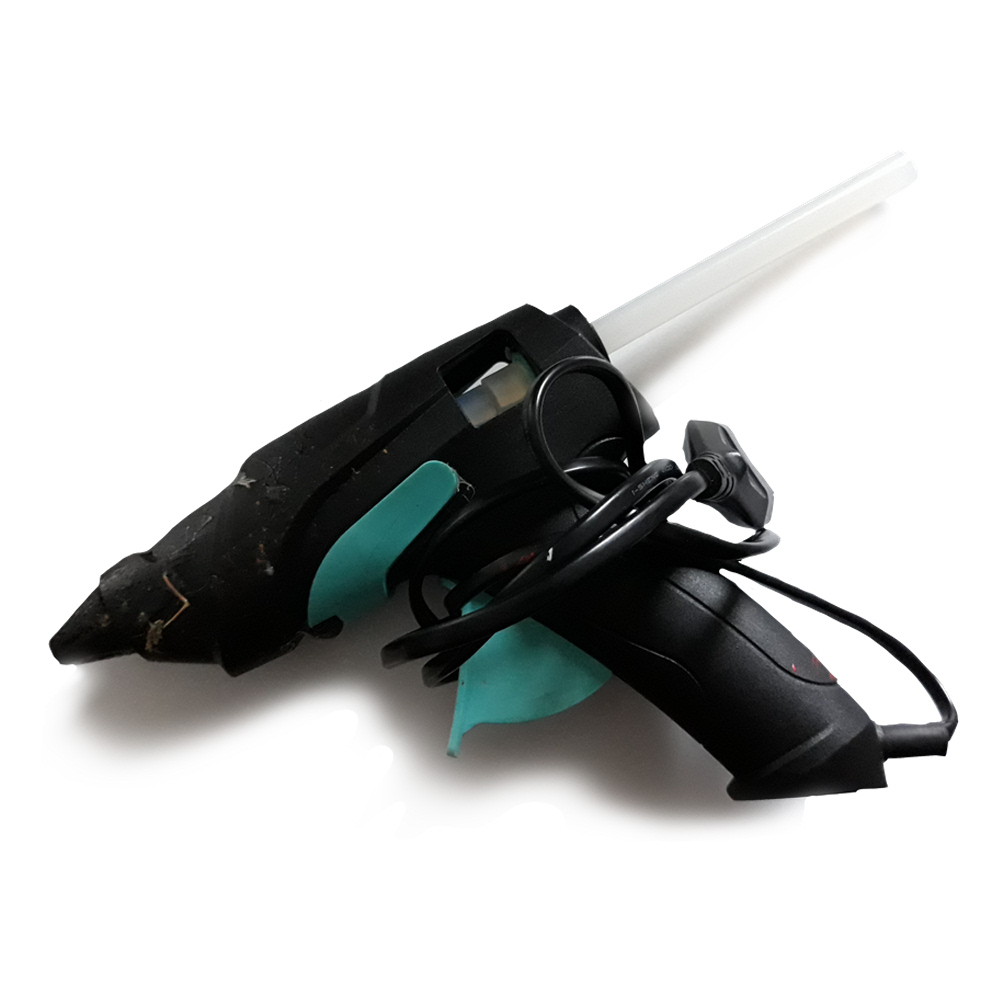
\includegraphics[width=5cm]{kleber.jpg}
\caption*{Heißklebepistole}
}
\qquad
\begin{minipage}{5cm}
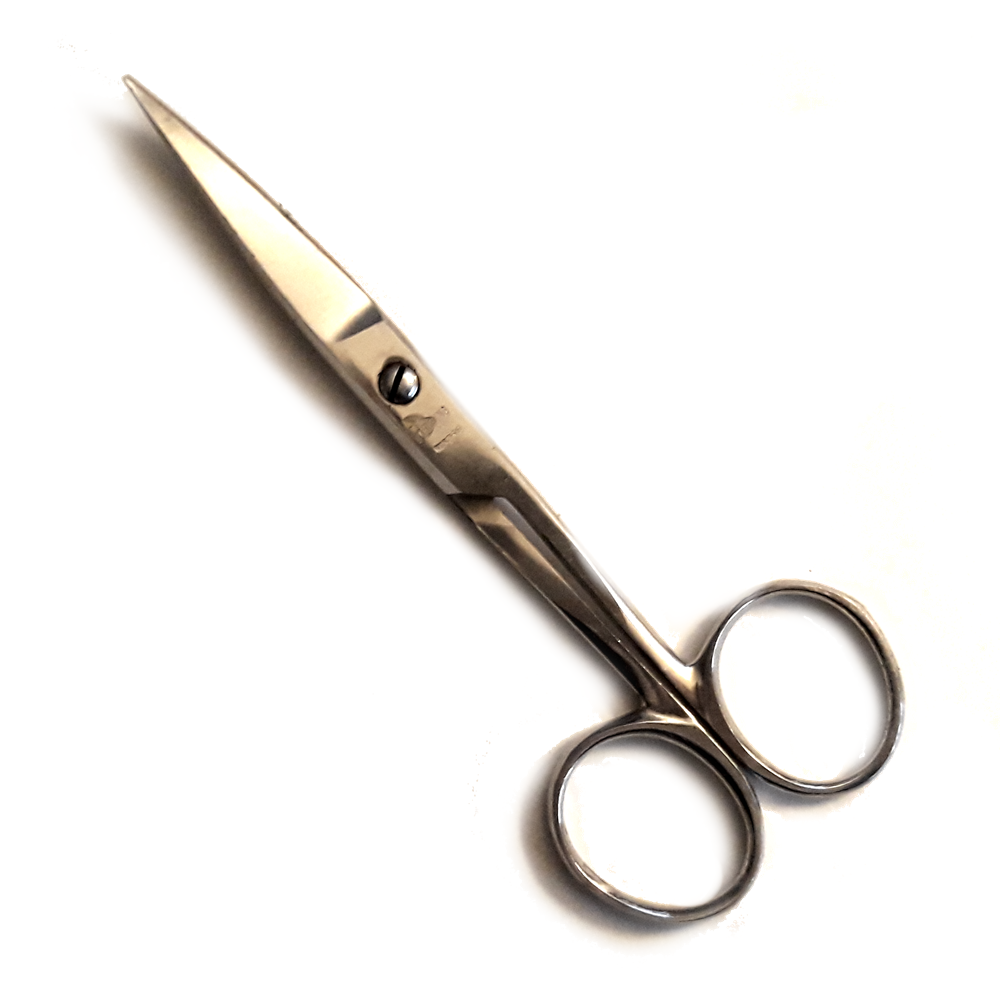
\includegraphics[width=5cm]{scheere.jpg}
\caption*{Schere}
\end{minipage}
\end{figure}
%%%%%%%%%%%%%%%%%%%%%%%%%%%%%%%%%%%%%%%%%%%%%%%%%

%%%%%%%%%%%%%%%%%%%%%%%%%%%%%%%%%%%%%%%%%%%%%%%%%
\begin{figure}[h]
\centering
\parbox{5cm}{
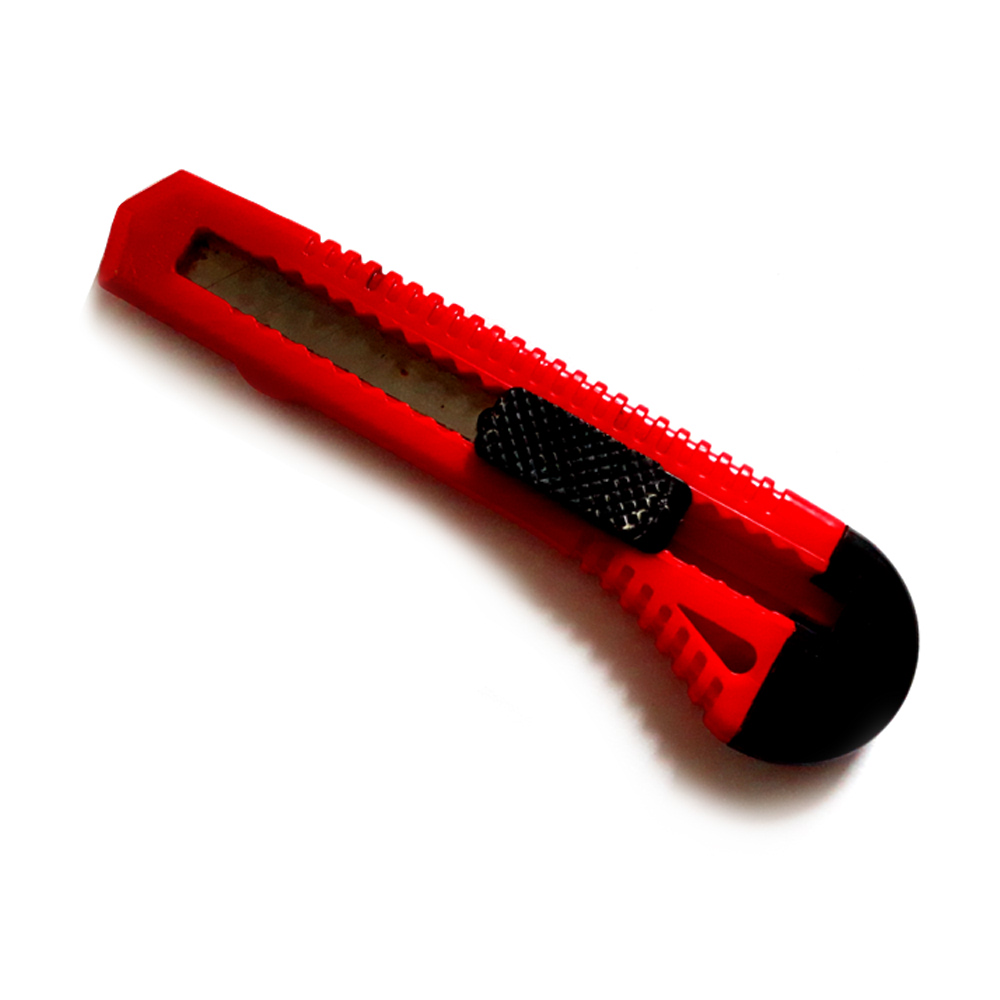
\includegraphics[width=5cm]{messer.jpg}
\caption*{Cuttermesser}
}
\qquad
\begin{minipage}{5cm}
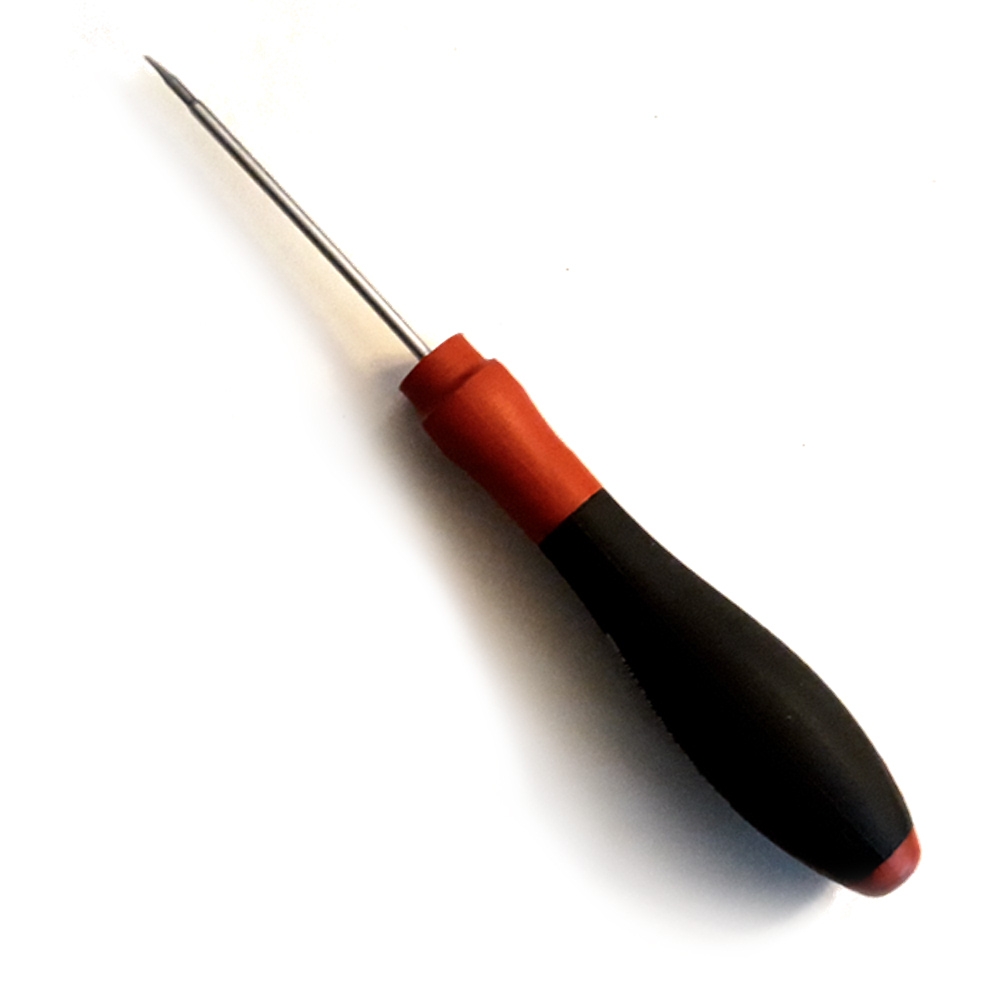
\includegraphics[width=5cm]{dreher.jpg}
\caption*{Schraubendreher}
\end{minipage}
\end{figure}
%%%%%%%%%%%%%%%%%%%%%%%%%%%%%%%%%%%%%%%%%%%%%%%%%
\begin{checklist}
    \item Heißklebepistole
    \item Schere / Teppichmesser
    \item Schraubenzieher

    \begin{checklist}
    \item[] Optional:
    \item Abisolierzange
    \item Lötkolben
    \end{checklist}
\end{checklist}

\subsubsection{Material}

%%%%%%%%%%%%%%%%%%%%%%%%%%%%%%%%%%%%%%%%%%%%%%%%%
\begin{figure}[h]
\centering
\parbox{5cm}{
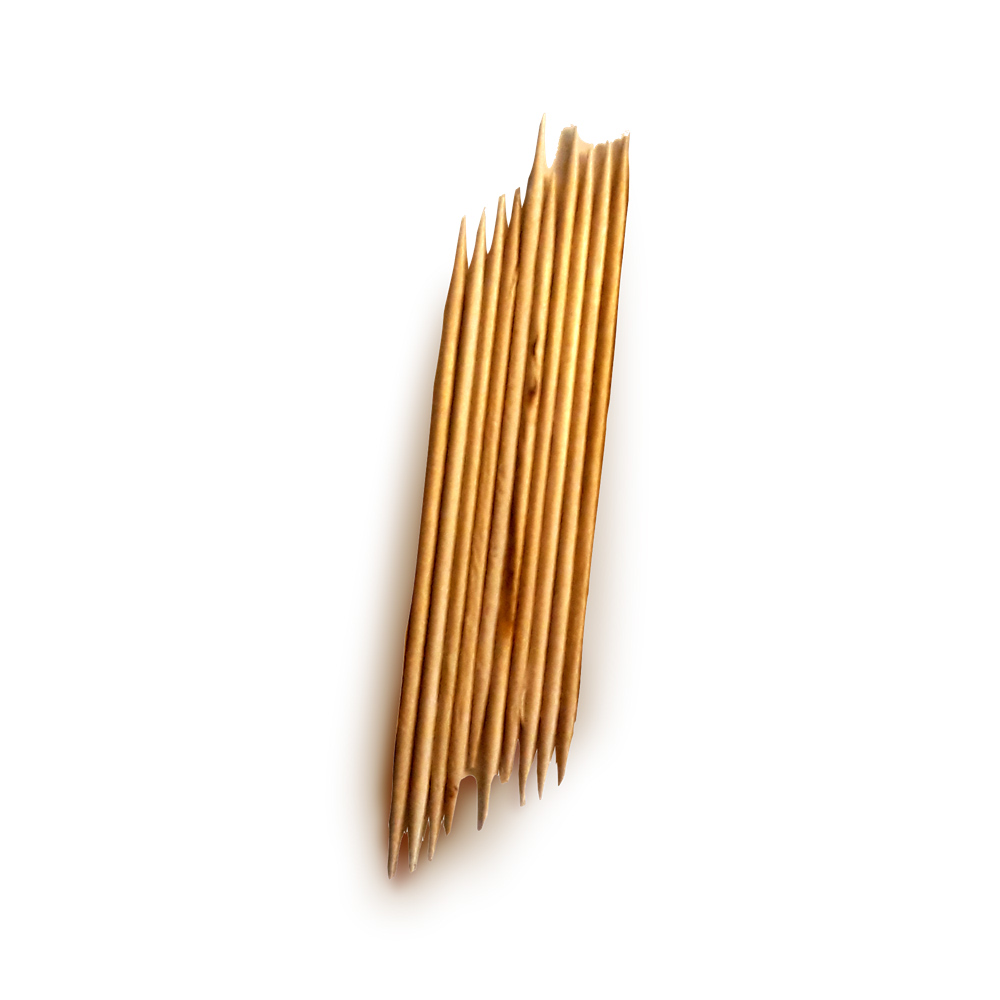
\includegraphics[width=5cm]{zahnstocher.jpg}
\caption*{Zahnstocher}
}
\qquad
\begin{minipage}{5cm}
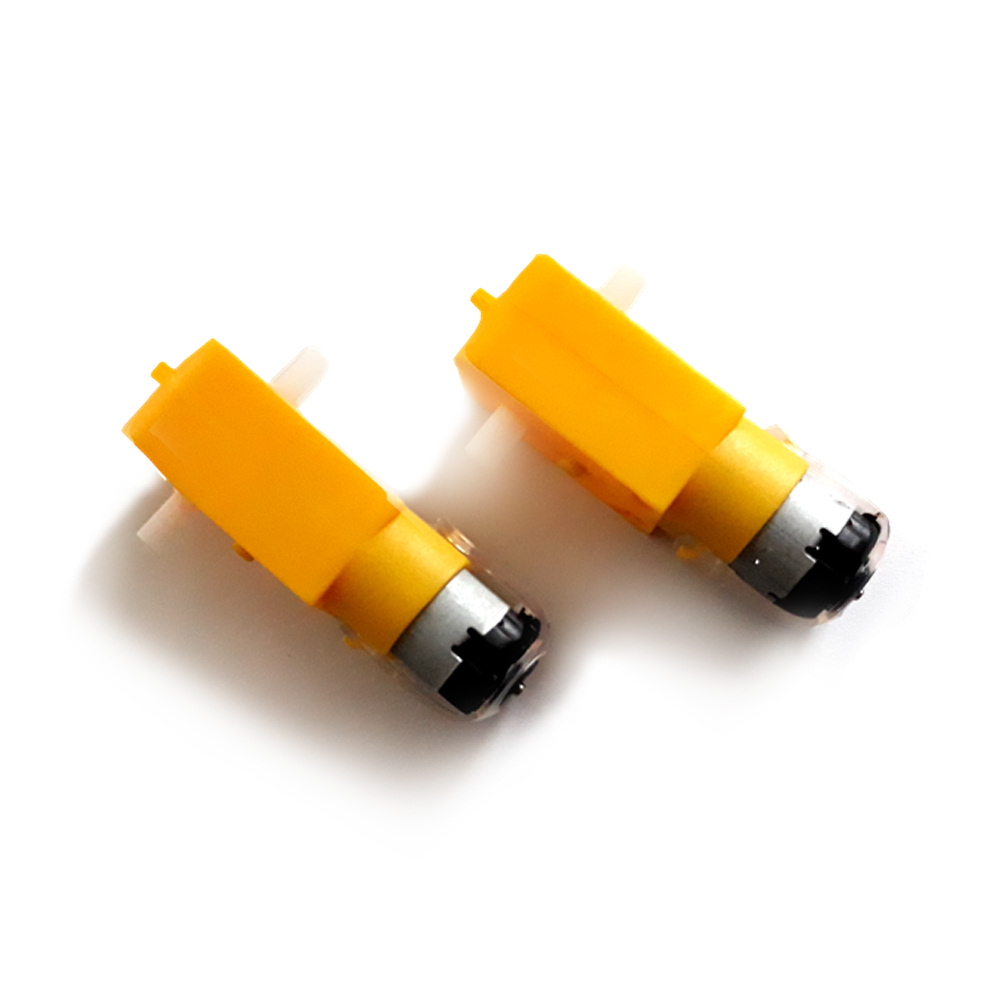
\includegraphics[width=5cm]{motoren.jpg}
\caption*{Motoren}
\end{minipage}
\end{figure}
%%%%%%%%%%%%%%%%%%%%%%%%%%%%%%%%%%%%%%%%%%%%%%%%%

%%%%%%%%%%%%%%%%%%%%%%%%%%%%%%%%%%%%%%%%%%%%%%%%%
\begin{figure}[h]
\centering
\parbox{5cm}{
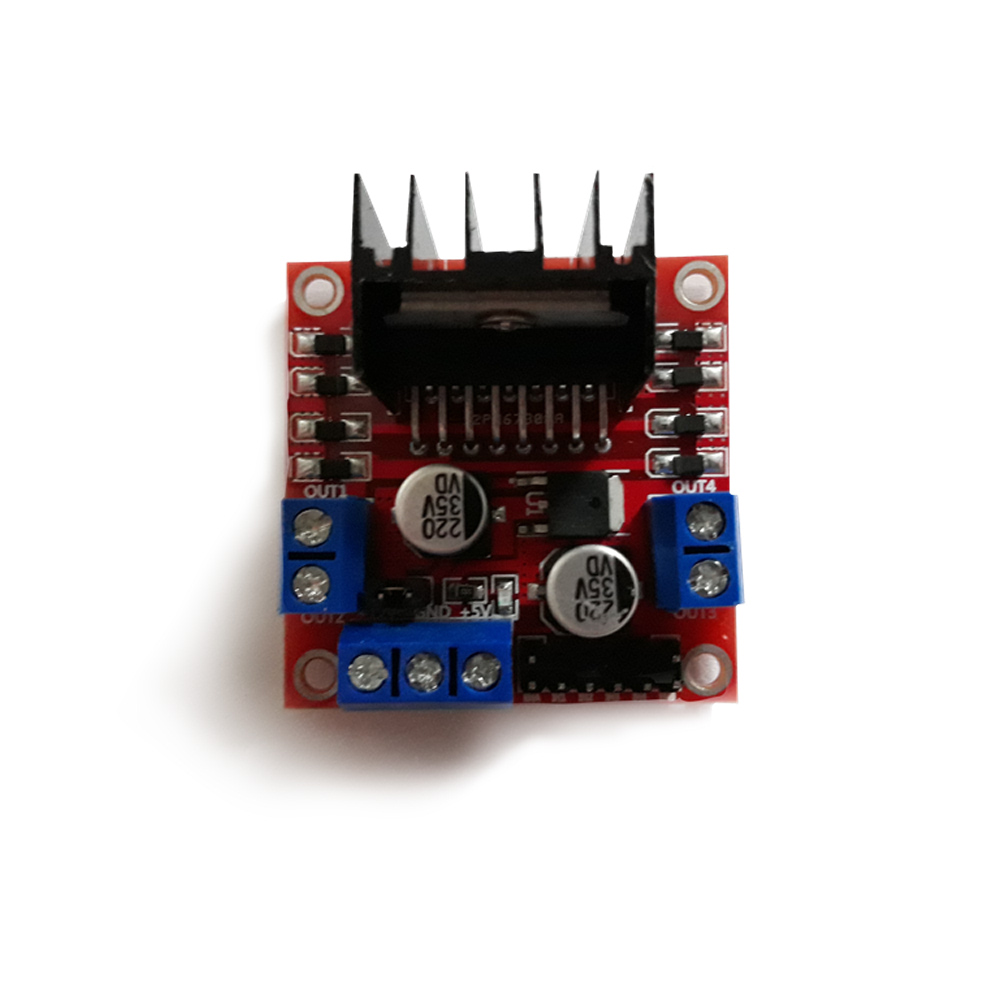
\includegraphics[width=5cm]{treiber.jpg}
\caption*{L298N Motortreiber - Erweiterung für den Raspberry-Pi}
}
\qquad
\begin{minipage}{5cm}
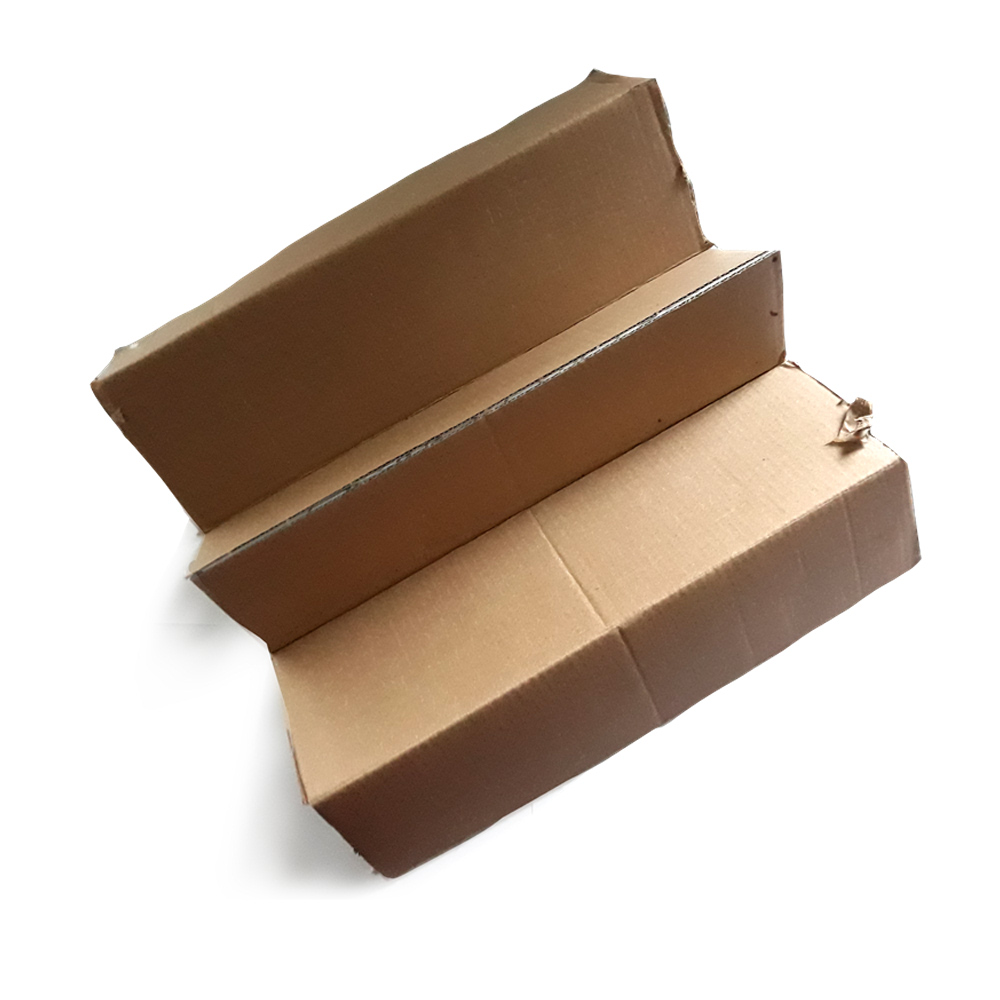
\includegraphics[width=5cm]{pappe.jpg}
\caption*{Ein Stück Pappe (mind. 30cm x 15cm}
\end{minipage}
\end{figure}
%%%%%%%%%%%%%%%%%%%%%%%%%%%%%%%%%%%%%%%%%%%%%%%%%

%%%%%%%%%%%%%%%%%%%%%%%%%%%%%%%%%%%%%%%%%%%%%%%%%
\begin{figure}[h]
\centering
\parbox{5cm}{
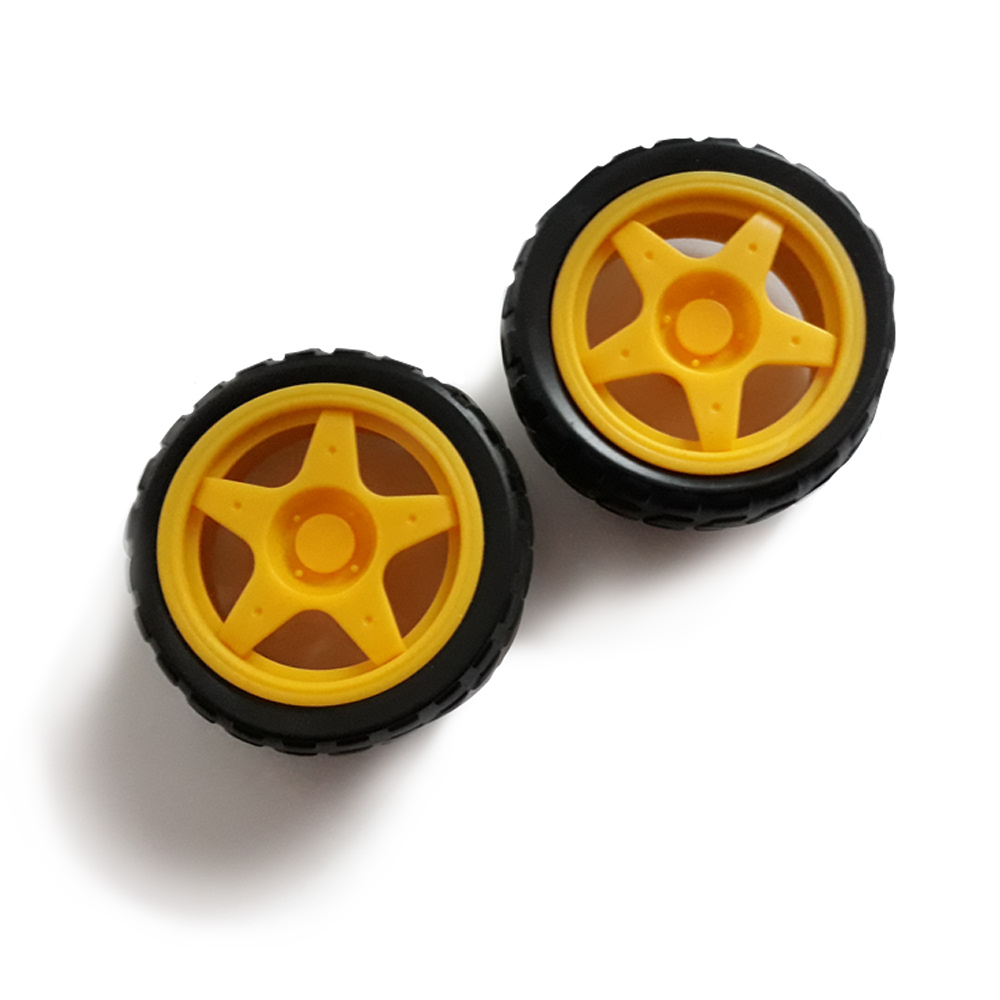
\includegraphics[width=5cm]{räder.jpg}
\caption*{Räder}
}
\qquad
\begin{minipage}{5cm}
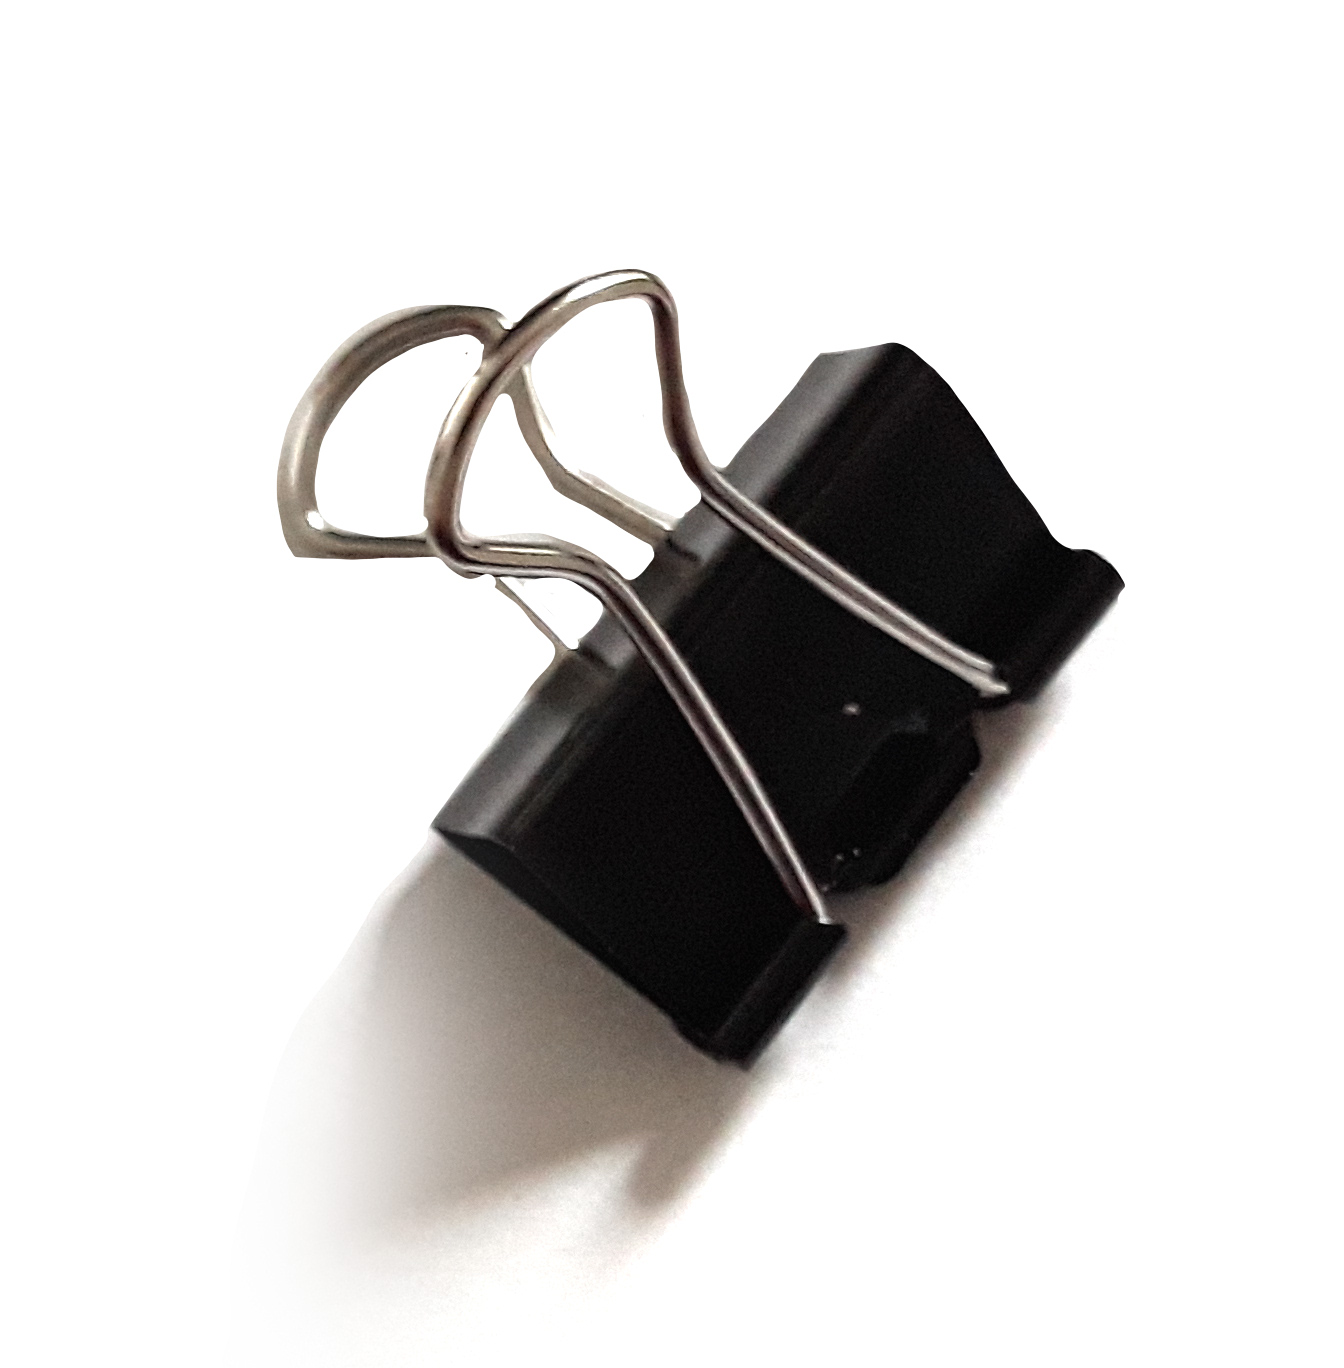
\includegraphics[width=5cm]{klammer.jpg}
\caption*{Maulklemme}
\end{minipage}
\end{figure}
%%%%%%%%%%%%%%%%%%%%%%%%%%%%%%%%%%%%%%%%%%%%%%%%%

%%%%%%%%%%%%%%%%%%%%%%%%%%%%%%%%%%%%%%%%%%%%%%%%%
\begin{figure}[h]
\centering
\parbox{5cm}{
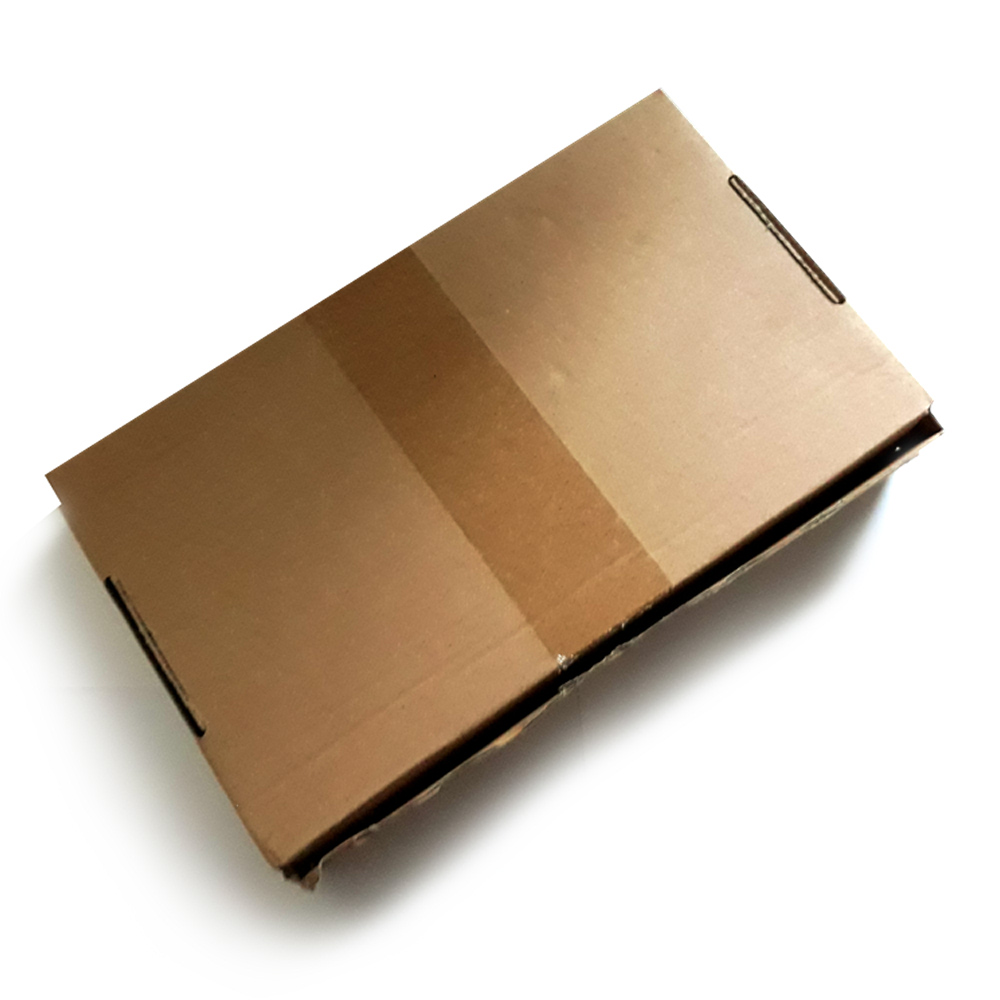
\includegraphics[width=5cm]{karton.jpg}
\caption*{Unterlage (Karton oder ein altes schweres Buch)}
}
\qquad
\begin{minipage}{5cm}
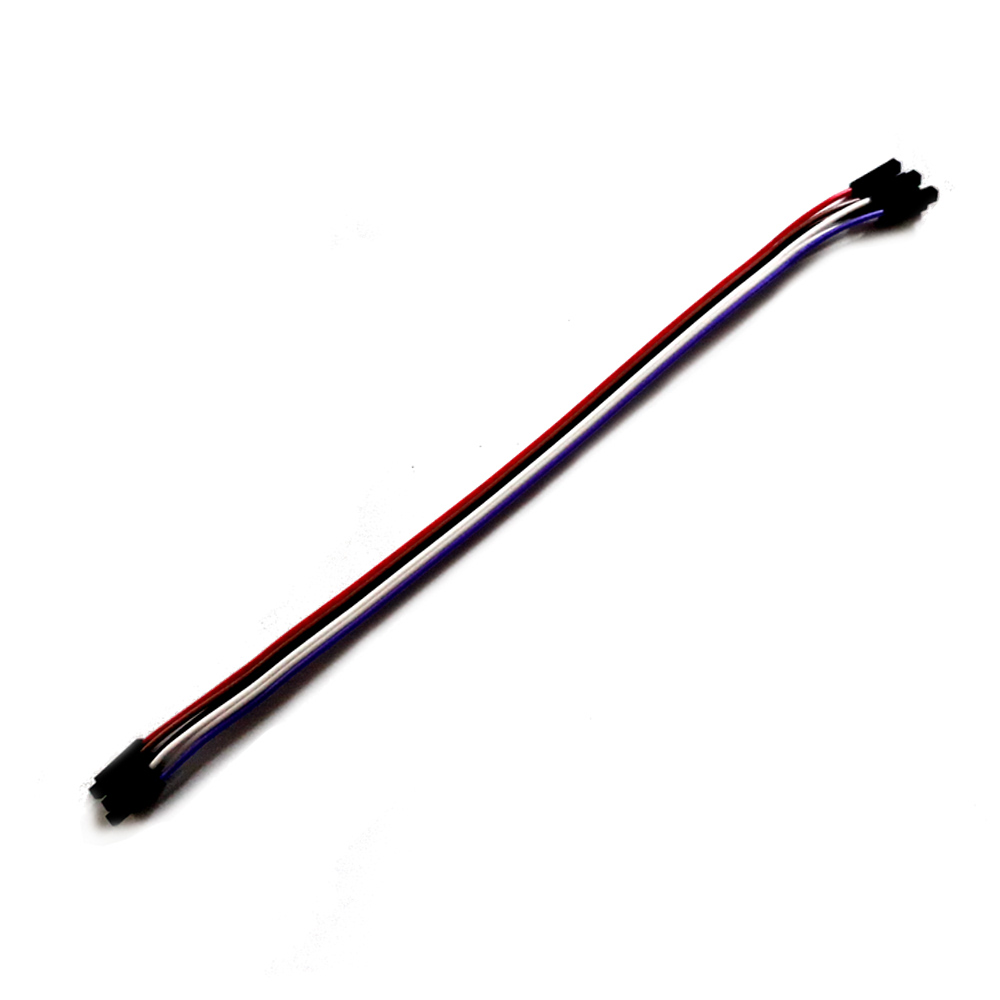
\includegraphics[width=5cm]{kabel ff.jpg}
\caption*{Female-Female Jumperkabel}
\end{minipage}
\end{figure}
%%%%%%%%%%%%%%%%%%%%%%%%%%%%%%%%%%%%%%%%%%%%%%%%%

%%%%%%%%%%%%%%%%%%%%%%%%%%%%%%%%%%%%%%%%%%%%%%%%%
\begin{figure}[h]
\centering
\parbox{5cm}{
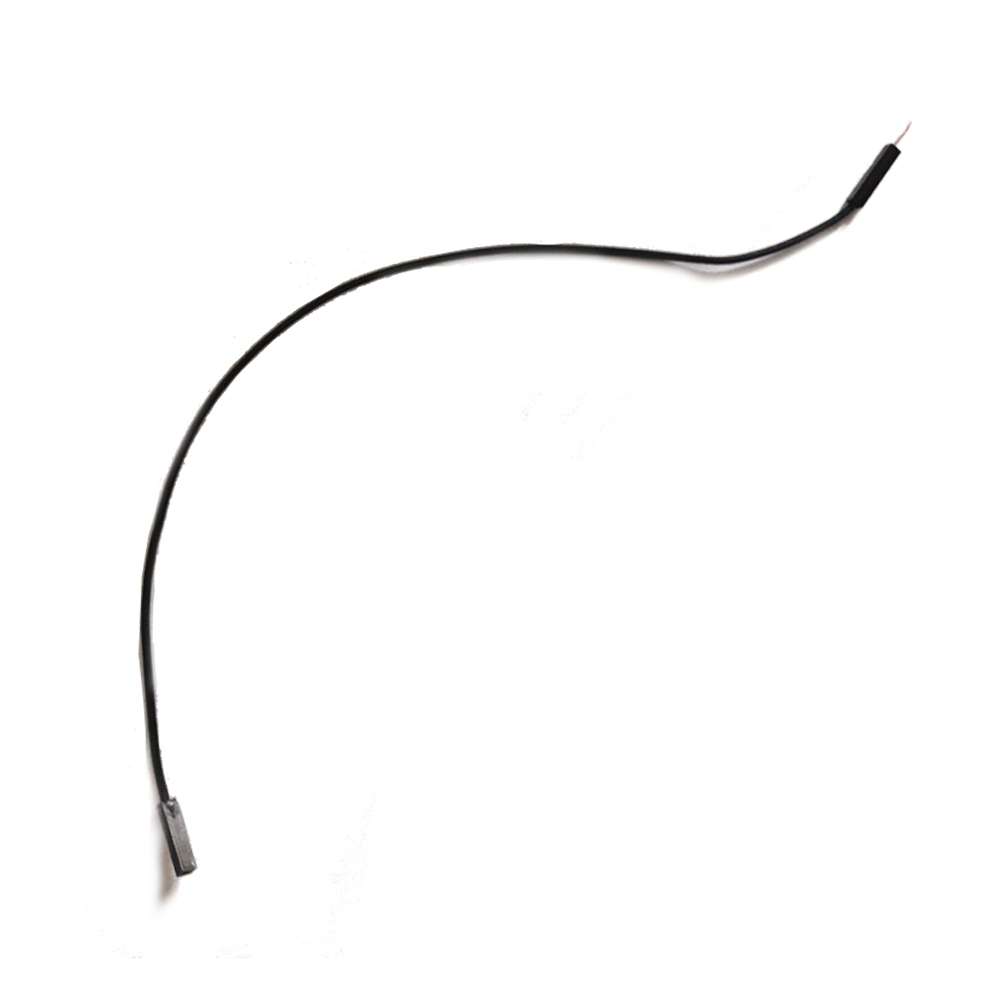
\includegraphics[width=5cm]{kabel male female.jpg}
\caption*{Stifte}
}
\qquad
\begin{minipage}{5cm}
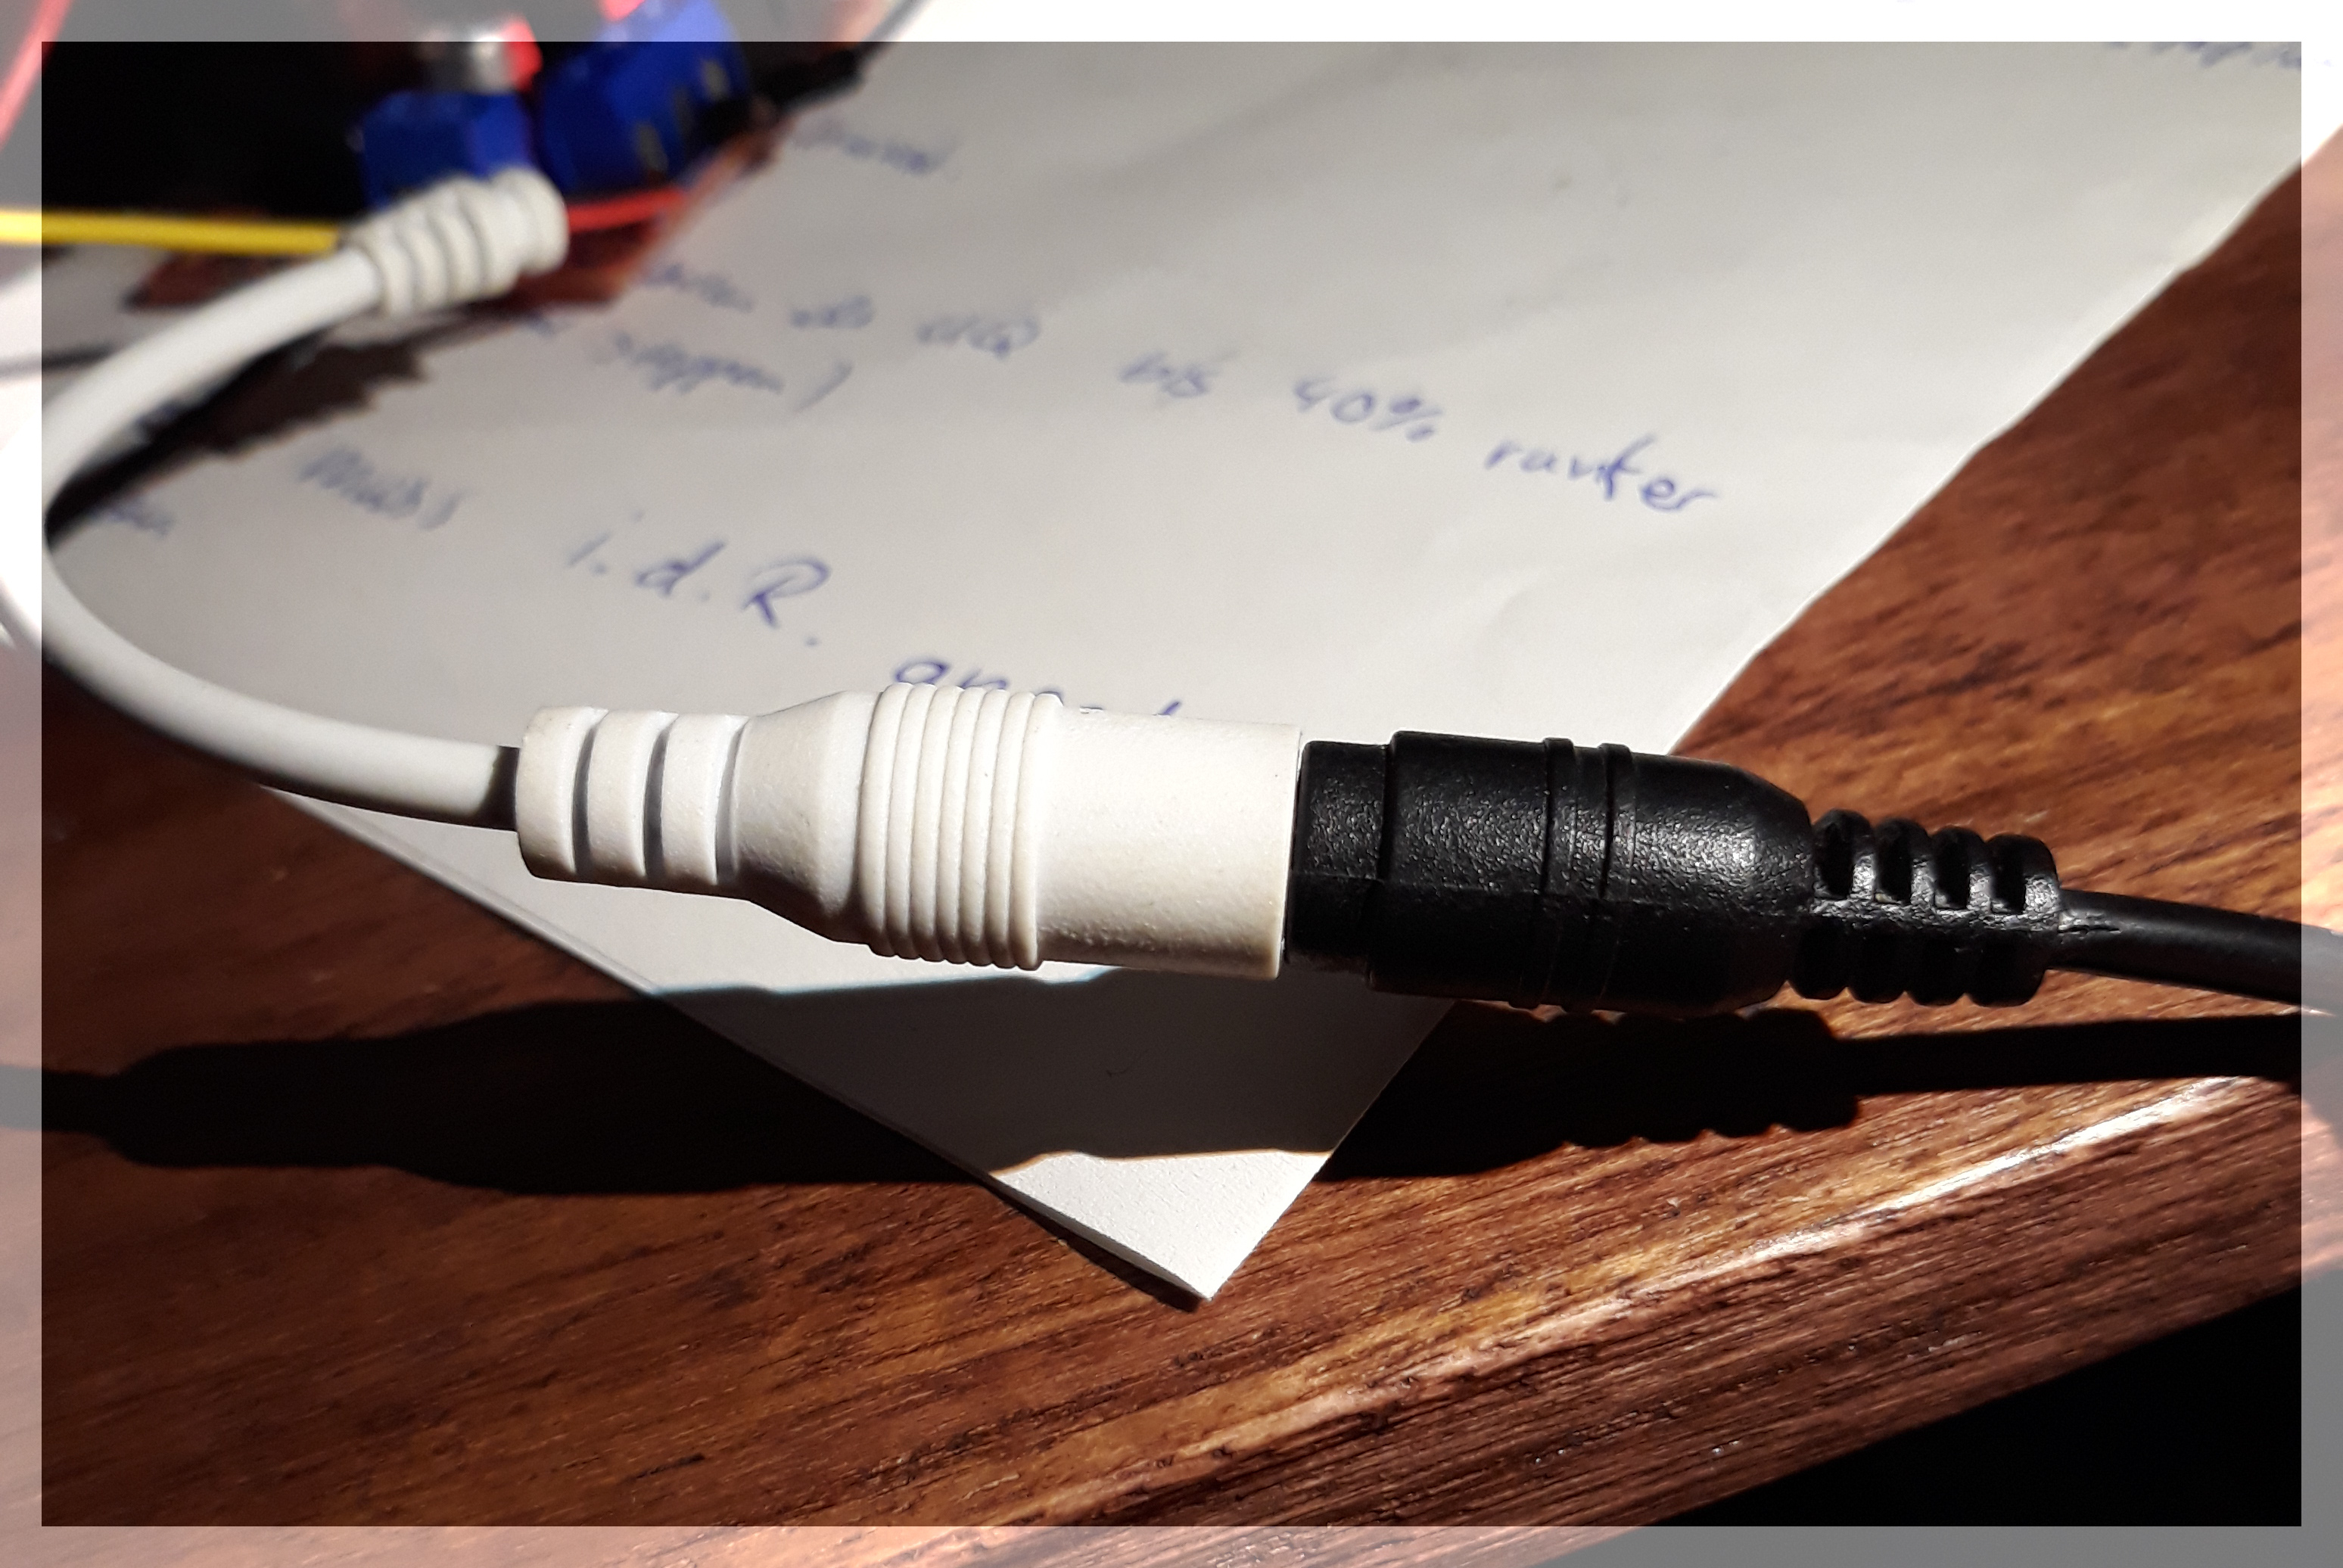
\includegraphics[width=5cm]{netzteil_close.jpg}
\caption*{Verbindungsstück von Netzteil und Adapter}
\end{minipage}
\end{figure}
%%%%%%%%%%%%%%%%%%%%%%%%%%%%%%%%%%%%%%%%%%%%%%%%%


\begin{checklist}
    \item RaspberryPi
    \item Bildschirm + HDMI-Kabel
    \item Maus + Tastatur
    \item Zahnstocher
    \item Motoren
    \item L298N Motortreiber
    \item Pappe
    \item 4x Kabel
    \item Räder
    \item Maulklemmen
    \item Unterlage (Telefonbuch / Karton)
    \item 6x Female-Female Jumperkabel
    \item 1x Female-Male Jumperkabel
    \item 12 V Netzteil und Adapter
\end{checklist}


\subsection{Software}
Auf dem RaspberryPi sollte bereits ein funktionierendes \emph{Betriebssystem} installiert sein. Dafür bietet sich \emph{Raspberry Pi OS} (Raspbian) an. \\

Bei dem ursprünglichen Projekt wurde die Programmierumgebung \emph{Scratch} verwendet, allerdings ist die Ansteuerung von Motoren mit Scratch auf dem Raspberry Pi  unnötig kompliziert. Deshalb sind wir hier auf die Verwendung der Programmiersprache \emph{Python} ausgewichen. Python bietet zwar keine grafische Programmieroberfläche wie Scratch, ist jedoch (nach Meinung der Autoren) eine für alle Altersgruppen intuitive und mindestens genauso zugängliche Programmiermethode.\\

Zur Ausführung der Python-Skripte eignet sich eine Entwicklungsumgebung, wie z.B. \emph{Thonny}, die auf dem Pi sogar schon vorinstalliert ist.\\
Vorkenntnisse über Python sind dabei hilfreich, aber nicht zwingend notwendig.

\subsubsection{Script}
Zur Vorbereitung sollten einige Funktionalitäten innerhalb von Python eingebaut werden, welche die Verwendung bei der Projektdurchführung für die KursteilnehmerInnen erleichtern.\\
Auf dem Raspberry Pi im Filmbüro sollten diese Dateien bereits vorhanden sein. Wenn das nicht der Fall ist, findet ihr im Anhang noch einmal eine ausführliche Erklärung mit den notwenigen Schritten am Ende der Dokumentation.\\


\subsection{Motoren}
Sollten die Motoren noch nicht mit Kabeln versehen sein, gibt es auch hierfür eine Anleitung im Anhang der Dokumentation.\\
Dieser Schritt lässt sich auch sehr gut mit den KursteilnehmerInnen durchführen!
